\vspace{-.2cm}
\section{Specific Graph Models}
\label{sec:examples}
\vspace{-.2cm}
Theorem~\ref{thm:main} shows that the effective resistance of the boundary plays a critical role in characterizing the distinguishability region of both the the GSS and LESS.
On specific graph families, we can compute the effective resistances precisely, leading to concrete detection guarantees that we will see nearly matches the lower bound in many cases.  Throughout this section, we will only be working with undirected, unweighted graphs.%, and we assume that $r_\Ccal = \omega(\sqrt {\log p})$.

Recall that Corollary~\ref{cor:main} shows that an SNR of $\omega\left(\sqrt{r_{\Ccal} \log p}\right)$ is sufficient while Theorem~\ref{thm:lower_bound} shows that $\Omega\left(\sqrt{\rho/d_{\max} \log p}\right)$ is necessary for detection.
Thus if we can show that $r_{\Ccal} \approx \rho/d_{\max}$, we would establish the near-optimality of both the GSS and LESS. 
Foster's theorem lends evidence to the fact that the effective resistances should be much smaller than the cut size:
\begin{theorem}(Foster's Theorem \cite{foster1949average,tetali1991random})
\[
\sum_{e \in E}r_e = p-1
\]
\label{thm:foster}
\end{theorem}
\vspace{-.5cm}
Roughly speaking, the effective resistance of an edge selected uniformly at random is $\approx (p-1)/m = d_{\textrm{ave}}^{-1}$ so the effective resistance of a cut is $\approx \rho/d_{\textrm{ave}}$.
This intuition can be formalized for specific models and this improvement by the average degree bring us much closer to the lower bound. 
\vspace{-.2cm}
\subsection{Edge Transitive Graphs}
An edge transitive graph, $G$, is one for which there is a graph automorphism mapping $e_0$ to $e_1$ for any pair of edges $e_0, e_1$. 
Examples include the $l$-dimensional torus, the cycle, and the complete graph $K_p$.
The existence of these automorphisms implies that every edge has the same effective resistance, and by Foster's theorem, we know that these resistances are exactly $(p-1)/m$. 
Moreover, since edge transitive graphs must be $d$-regular, we know that $m = \Theta(pd)$ so that $r_e = \Theta(1/d)$.
Thus as a corollary to Theorem~\ref{thm:main} we have that both the GSS and LESS are near-optimal (optimal modulo logarithmic factors whenever  $\rho/d \le \sqrt{p}$) on edge transitive graphs:
\begin{corollary}
Let $G$ be an edge-transitive graph with common degree $d$. Then both the GSS and LESS distinguish $H_0$ from $H_1$ provided that:
\[
\mu = \omega\left(\max\{\sqrt{\rho/d \log p}, \log p\}\right)
\]
\label{cor:edge_trans}
\end{corollary}
\vspace{-.75cm}
\subsection{Random Geometric Graphs}
Another popular family of graphs are those constructed from a set of points in $\mathbb{R}^D$ drawn according to some density. 
These graphs have inherent randomness stemming from sampling of the density, and thus earn the name \emph{random geometric graphs}.
The two most popular such graphs are \emph{symmetric k-nearest neighbor graphs} and \emph{$\epsilon$-graphs}.
We characterize the distinguishability region for both. 

In both cases, a set of points $\zb_1, \ldots, \zb_p$ are drawn i.i.d. from a density $f$ support over $\mathbb{R}^D$, or a subset of $\mathbb{R}^D$. 
Our results require mild regularity conditions on $f$, which, roughly speaking, require that $\textrm{supp}(f)$ is topologically equivalent to the cube and has density bounded away from zero (See~\cite{vonluxburg2010} for a precise definition). 
To form a $k$-nearest neighbor graph $G_k$, we associate each vertex $i$ with a point $\zb_i$ and we connect vertices $i,j$ if $\zb_i$ is amongst the $k$-nearest neighbors, in $\ell_2$, of $\zb_j$ or vice versa.
In the the $\epsilon$-graph, $G_\epsilon$ we connect vertices $i,j$ if $||\zb_i - \zb_j|| \le \epsilon$ for some metric $\tau$. 

The relationship $r_e \approx 1/d$, which we used for edge-transitive graphs, was derived in Corollaries 8 and 9 in~\cite{vonluxburg2010}
%% As with the edge-transitive graph, we want to show that $r_e \approx 1/d$, and fortunately, this relationship was derived in Corollaries 8 and 9 in~\cite{vonluxburg2010}.
The precise concentration arguments, which have been done before~\cite{sharpnack2012detecting}, lead to the following corollary regarding the performance of the GSS and LESS on random geometric graphs:
\begin{corollary}
Let $G_k$ be a $k$-NN graph with $k/p \rightarrow 0$, $k(k/p)^{2/D} \rightarrow \infty$ and suppose the density $f$ meets the regularity conditions in~\cite{vonluxburg2010}.
Then both the GSS and LESS distinguish $H_0$ from $H_1$ provided that:
\[
\mu = \omega\left(\max\{\sqrt{\rho/k\log p},\log p\}\right)
\]
If $G_\epsilon$ is an $\epsilon$-graph with $\epsilon \rightarrow 0$, $n\epsilon^{D+2}\rightarrow \infty$ then both distinguish $H_0$ from $H_1$ provided that:
\[
\mu = \omega\left(\max \left\{\sqrt{\frac{\rho}{p\epsilon^D} \log p}, \log p\right \}\right)
\]
\end{corollary}
The corollary follows immediately form Corollary~\ref{cor:main} and the proofs in~\cite{sharpnack2012detecting}.
Since under the regularity conditions, the maximum degree is $\Theta(k)$ and $\Theta(p\epsilon^D)$ in $k$-NN and $\epsilon$-graphs respectively, the corollary establishes the near optimality (again provided that $\rho/d \le \sqrt{p}$) of both test statistics.

\begin{figure}[t]
\begin{center}
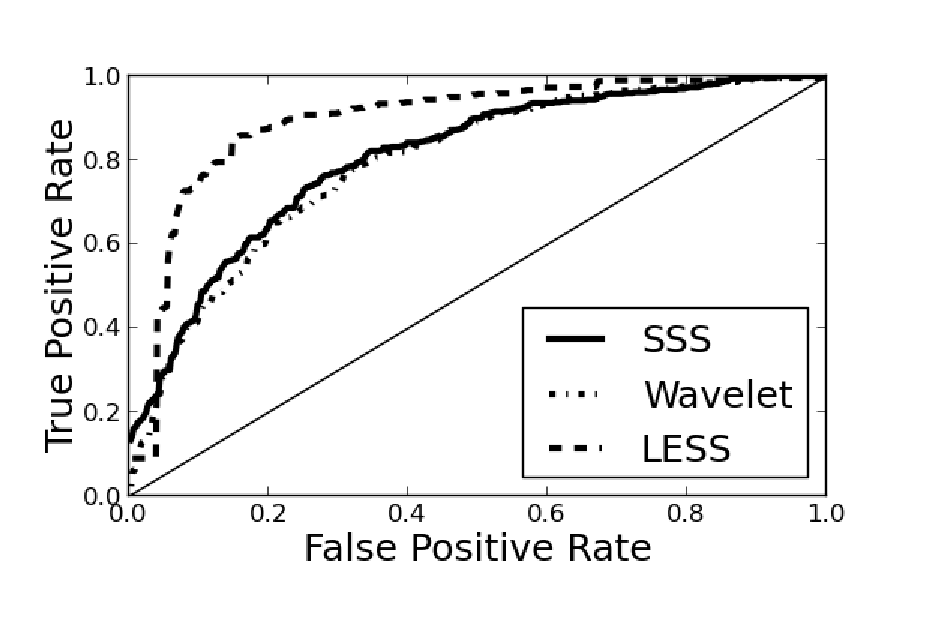
\includegraphics[width=4.5cm]{tor_n=225_mu=4.eps}
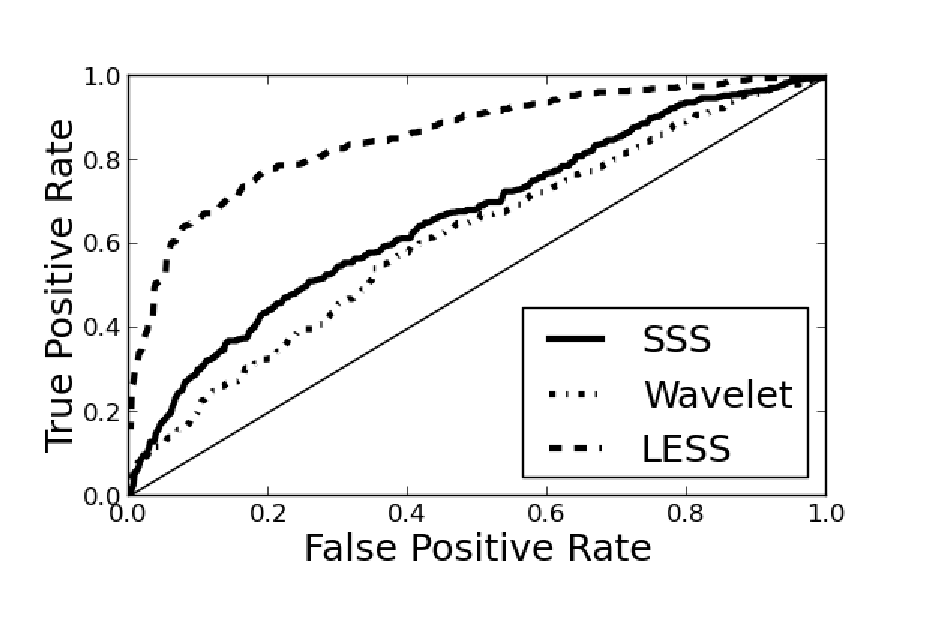
\includegraphics[width=4.5cm]{knn_n=225_mu=4.eps}
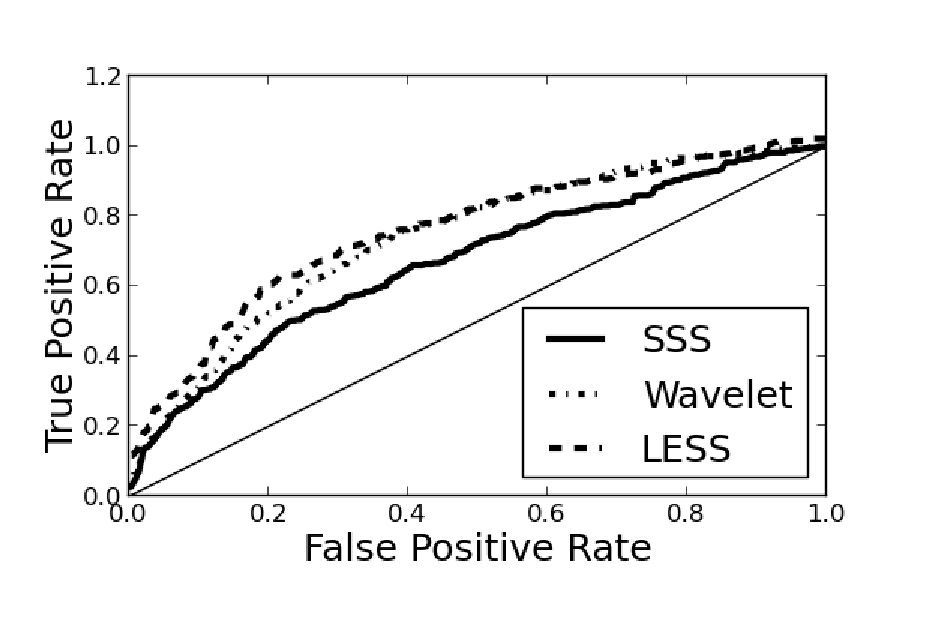
\includegraphics[width=4.5cm]{eps_n=225_mu=3.eps}
\end{center}
\caption{A comparison of detection procedures: spectral scan statistic (SSS), UST wavelet detector (Wavelet), and LESS.  The graphs used are the square 2D Torus, kNN graph ($k \approx p^{1/4}$), and $\epsilon$-graph (with $\epsilon \approx p^{-1/3}$); with $\mu = 4,4,3$ respectively, $p = 225$, and $|C| \approx p^{1/2}$.}
\vspace{-.2cm}
\end{figure}
We performed some experiments using the MRF based algorithm outlined in Prop.~\ref{prop:less_alg}.
Each experiment is made with graphs with $225$ vertices, and we report the true positive rate versus the false positive rate as the threshold varies (also known as the ROC.)
For each graph model, LESS provides gains over the spectral scan statistic\cite{sharpnack2012changepoint} and the UST wavelet detector\cite{sharpnack2012detecting}, each of the gains are significant except for the $\epsilon$-graph which is more modest.
\vspace{-.2cm}
\section{Conclusions}
\vspace{-.2cm}
To summarize, while Corollary~\ref{cor:main} characterizes the performance of GSS and LESS in terms of effective resistances, in many specific graph models, this can be translated into near-optimal detection guarantees for these test statistics.
We have demonstrated that the LESS provides guarantees similar to that of the computationally intractable generalized likelihood ratio test (GSS).
Furthermore, the LESS can be solved through successive graph cuts by relating it to MAP estimation in an MRF.
Future work includes using these concepts for localizing the activation, making the program robust to missing data, and extending the analysis to non-Gaussian error.
\vspace{-.2cm}
%This procedure is very flexible as it applies to weighted and directed graphs, which to the best of our knowledge is the first instance of a anomaly detection algorithm that works for directed graphs with statistical guarantees.


